\documentclass[10pt]{article}
\usepackage{amssymb}
\usepackage{graphicx}
\usepackage{verbatim}
\usepackage{graphicx}
\usepackage{fontspec}
\usepackage{longtable}
\usepackage{tabulary}
\usepackage{xtab}
\usepackage[table]{xcolor}
\usepackage{geometry}

\geometry{a4paper, top=2.5cm, bottom=2.5cm, left=2cm, right=2cm}

\setmainfont{Arial}
\graphicspath{ {./images/} }

\title{
    \begin{center}
        \textbf{GrandeSlam} \\
       \small Relazione progetto Basi di Dati
    \end{center}
}
\author{Davide Sut}
\date{Anno accademico 2020-2021}

\setlength\parindent{0pt}

\newcommand{\spazia}{\par\medskip}
\newcommand{\splitcell}[2][l]{%
  \begin{tabular}[l]{@{}l@{}}\strut#2\strut\end{tabular}%
}

\begin{document}

\maketitle
\pagebreak
\section{Abstract}
\textit{GrandeSlam} è un'organizzazione che si occupa della vendita online di biglietti per i maggiori tornei nazionali ed internazionali di tennis tramite il proprio sito.

L'organizzazione ha inoltre l'intento di mettere a disposizione degli appassionati le informazioni dettagliate delle partite e tornei già disputati e di quelli in corso.

Una volta registrati, gli utenti possono ricercare e consultare le informazioni relative ai tornei: classificazione ATP, tipo di terreno di gioco, tennisti in gara, ranking, percentuali di successo, etc..

Possono inoltre procedere all'acquisto di uno o più biglietti inserendoli nel carrello e procedendo all'ordine fornendo una modalità di pagamento valida che non verrà memorizzata nel database per non violare la privacy degli utenti.


\section{Analisi dei Requisiti}

\subsection{Descrizione dei requisiti}
Il progetto vuole rappresentare una base di dati per la gestione delle informazioni riguardanti i principali tornei di tennis e degli ordini effettuati dagli utenti.\spazia

Nella base di dati le persone vengono divise in tennisti, giudici e utenti, che a loro volta possono essere amministratori.

Due tennisti possono formare una coppia: si parlerà genericamente di giocatore, per intendere un tennista o una coppia.

I tennisti e i giudici vengono inseriti da un amministratore del sito, mentre gli utenti devono registrarsi e fornire nome, cognome, data di nascita, sesso e un indirizzo email inizialmente opzionale, ma che diventa obbligatorio con il primo ordine nel sito.\spazia

Gli utenti, una volta registrati, possono aggiungere uno o più biglietti all'interno del proprio carrello e poi procedere all'ordine per acquistarli.

Ciascun biglietto include una o più partite nell'arco di una sola giornata.\spazia

Gli utenti del sito, inoltre, possono avere accesso a tutte le statistiche e allo storico delle edizioni dei tornei e delle partite di qualsiasi tennista o coppia che gioca a livello competitivo.\spazia

I tornei sono organizzati dalle federazioni tennistiche ATP, WTA e ITF: ATP gestisce i tornei maschili, WTA quelli femminili e ITF entrambi.

Si occupano dell'organizzazione anche le società tennistiche del paese in cui si gioca, le quali mettono a disposizione la struttura con i vari campi.

Ogni torneo ha degli sponsor, tra cui solitamente uno principale che aiuta economicamente la società tennistica che lo organizza.\spazia

I tornei dello stesso livello fanno parte di un Tour che si ripete ogni anno con qualche piccola variazione. 

Esistono principalmente 3 tipi di Tour: ATP e WTA Tour, ATP e WTA Challenger Tour e ITF Tour, rispettivamente di primo, secondo e terzo livello.\spazia

All'interno dei Tour, i tornei vengono ulteriormente divisi in base ai punti ranking massimi che assegnano e che corrispondono alla vittoria del torneo. 

Ad esempio, l'ATP Tour è diviso in  ATP World Tour Masters 1000, ATP World Tour 500 series, ATP World Tour 250 series, dove 1000, 500 e 250 sono i punti ranking assegnati al vincitore.

A questi tornei si aggiungono i 4 tornei del Grande Slam, i più importanti, che assegnano 2000 punti ranking al vincitore: US Open, Australian Open, Roland Garros e Wimbledon.\spazia

Ai giocatori iscritti al torneo vengono comunque associati dei punti ranking, in base alla fase in cui hanno disputato l'ultima partita.

Inoltre, molti tornei oltre ad essere giocati in singolo, possono anche essere giocati in doppio, ovvero da una coppia di tennisti. 

I punti ranking del doppio si differenziano da quelli in singolo e vanno a comporre una classifica diversa.\spazia

Le partite si disputano solitamente al meglio di 3 o 5 set per gli uomini e al meglio di 3 set per le donne.\spazia

Le partite vengono disputate in un campo con più o meno spettatori in base all'importanza dei giocatori e alla fase del torneo.

In una giornata possono essere programmate anche più partite nello stesso campo, una di seguito all'altra.\spazia

Viene infine offerta anche la possibilità di vedere il risultato di una partita di tennis in diretta con relative statistiche, la programmazione delle partite successive riguardanti un determinato torneo e il tabellone di una qualsiasi edizione di un torneo aggiornato alla fase attuale.\spazia


\subsection{Glossario dei termini}

\begin{xtabular}[H]{|p{2.3cm}|p{7.5cm}|p{4.35cm}|}
    \hline
    \rowcolor{lightgray} \textbf{Termine} & \textbf{Descrizione} & \textbf{Collegamenti}  \\
    \hline
    Biglietto & Biglietto per una partita di tennis & \splitcell{Collegata con Partita, \\ Ordine, Utente} \\
    \hline
    Campo & Luogo dove si disputa una partita & \splitcell{Collegata con Partita,\\ Torneo} \\
    \hline
    Ordine & \splitcell{Insieme di biglietti acquistati da un utente} & \splitcell{Collegata con Biglietto,\\ Utente} \\
    \hline
    Partita & Partita di tennis disputata o da disputarsi & \splitcell{Collegata con Edizione \\torneo, Giocatore, Campo,\\ Statistiche, Giudice di\\ sedia, Biglietto, Partita, \\Dettaglio partita} \\
    \hline
    \splitcell{Dettaglio \\partita} & \splitcell{Informazioni aggiuntive riguardanti una specifica \\partita di tennis} & \splitcell{Collegata con Partita} \\
    \hline
    Persona & \splitcell{Tennisti, giudici di sedia e utenti presenti nel sito}.  & \splitcell{Entità padre di Tennista,\\ Giudice di sedia e Utente}\\
    \hline
    Utente & \splitcell{Persona che può acquistare un biglietto nel sito \\e visualizzare le informazioni dettagliate delle\\ partite e tornei di tennis} & \splitcell{Entità figlia di Persona\\
    Collegata con Ordine e \\ Biglietto} \\
    \hline
    Amministratore & \splitcell{Utente dotato di privilegi speciali la cui funzione\\ è amministrare il sito } & Entità figlia di Utente \\
    \hline
    \splitcell{Giudice \\di sedia} & Persona che arbitra le partite di tennis & \splitcell{Entità figlia di Persona\\ Collegata con Partita} \\
    \hline
    Giocatore & Tennista o coppia iscritta ad un torneo di tennis & \splitcell{Entità padre di Tennista e\\ Coppia\\Collegata con Partita, \\Edizione torneo, Statistiche} \\
    \hline
    Tennista & \splitcell{Persona che può iscriversi ad un torneo come\\ giocatore singolo} & \splitcell{Entità figlia di Giocatore e\\ Persona\\Collegata con Coppia} \\
    \hline
    Coppia & \splitcell{Insieme di due tennisti che può iscriversi ad un\\ torneo come coppia} & \splitcell{Entità figlia di Giocatore\\Collegata con Tennista} \\
    \hline
    \splitcell{Società \\tennistica}& Ente che organizza uno o più tornei di tennis & Collegata con Torneo \\
    \hline
    Sponsor & Ente che sponsorizza uno o più tornei di tennis & Collegata con Torneo \\
    \hline
    Statistiche & \splitcell{Insieme di dati riguardanti un giocatore in una \\specifica partita} & \splitcell{Collegata con Partita e\\ Giocatore} \\
    \hline
    Torneo & \splitcell{Insieme di partite di tennis organizzate in fasi \\successive, in modo da far competere i vari \\vincitori fino alla finale, nella quale il vincente \\vince anche il torneo} & \splitcell{Collegata Sponsor, Società\\ tennistica, Edizione torneo, \\Campo}  \\
    \hline
    \splitcell{Edizione\\torneo} & \splitcell{Edizione di un torneo in un anno specifico} & \splitcell{Collegata con Partita,\\ Giocatore, Torneo} \\
    \hline
    ATP & \splitcell{Acronimo di \textit{Association of Tennis Professionals}\\ è un'associazione di tennis maschile che \\organizza tornei di tennis} & Attributo di Torneo \\
    \hline
    WTA & \splitcell{Acronimo di \textit{Women's Tennis Association} è un'\\associazione di tennis femminile che organizza \\tornei di tennis} & Attributo di Torneo \\
    \hline
    Challenger & \splitcell{Tipologia di tornei di tennis di secondo livello \\organizzati da ATP e WTA} & Attributo di Torneo \\
    \hline
    ITF & \splitcell{Acronimo di \textit{International Tennis Federation} è il\\ corpo dirigente del tennis mondiale, organizza \\i 4 tornei più importanti del tennis cioè quelli del \\Grande Slam e anche tornei più piccoli di terzo \\livello} & Attributo di Torneo \\
    \hline
    Singolo & \splitcell{Modalità di gioco del tennis in cui gareggia un\\ tennista contro un altro tennista} & Attributo di Partita e Torneo \\
    \hline
    Doppio &  \splitcell{Modalità di gioco del tennis in cui gareggia una\\ coppia di tennisti contro un'altra coppia} & Attributo di Partita e Torneo \\
    \hline
    Set & \splitcell{Gli incontri si suddividono in set. In base al tipo\\ di torneo, gli incontri sono al meglio di 3 o 5 set.\\ Sono composti da un certo numero di giochi} & Attributo di Dettaglio Partita \\
    \hline
    Giochi & \splitcell{I set si suddividono in giochi. Per ottenere un set,\\ bisogna conquistare almeno 6 giochi e avere un\\ distacco di almeno 2 giochi dall'avversario. Se il \\punteggio è di 6-6, solitamente si procede con il \\tie-break: il primo giocatore che conquista\\ almeno 7 punti con un distacco minimo di 2 \\ vince il gioco e quindi il set. \\Sono composti da un certo numero di punti} & Attributo di Dettaglio Partita \\
    \hline
    Punti & \splitcell{Nel tennis i punti vengono assegnati nella\\ successione di "15", "30", "40", "gioco" corrispon-\\denti a una successione di quattro punti conquis-\\tati. Se ci si trova nel punteggio di 40 - 40, si va \\ai vantaggi, dove vince il gioco il primo giocatore \\che ottiene due punti di vantaggio sull'avversario} & Attributo di Dettaglio Partita \\
    \hline
\end{xtabular}

\subsection{Strutturazione dei requisiti}

\begin{xtabular}{|p{\textwidth}|}
    \hline
    \rowcolor{lightgray} \multicolumn{1}{|c|}{Frasi relative a \textit{\textbf{GrandeSlam}}} \\ 
    \hline
    \textit{GrandeSlam} è un'organizzazione che si occupa della vendita online di biglietti per i maggiori tornei nazionali ed internazionali di tennis tramite il proprio sito.
    
    L'organizzazione ha inoltre l'intento di mettere a disposizione degli appassionati le informazioni dettagliate dei tornei già disputati e di quelli in corso. \\
    \hline
    \rowcolor{lightgray} \multicolumn{1}{|c|}{Frasi relative a \textbf{Biglietto}} \\ 
    \hline
    Possono inoltre procedere all’acquisto di uno o più biglietti inserendoli nel carrello e procedendo all’ordine fornendo una modalità di pagamento valida che non verrà memorizzata nel database per non violare la privacy degli utenti.[...] Gli utenti una volta registrati possono aggiungere uno o più biglietti all’interno del proprio carrello e poi procedere all’ordine per acquistarli.\newline
    I biglietti includono una o più partite nell’arco di una sola giornata.\\
    \hline
    \rowcolor{lightgray} \multicolumn{1}{|c|}{Frasi relative a \textbf{Campo}} \\ 
    \hline
    Le partite vengono disputate in un campo con più o meno spettatori in base all'importanza dei tennisti e della fase dell'eventuale torneo.\newline
    In una giornata possono essere programmate anche più partite nello stesso campo, una di seguito all'altra. \\
    \hline
    \rowcolor{lightgray} \multicolumn{1}{|c|}{Frasi relative a \textbf{Giocatore}} \\ 
    \hline
    Due tennisti possono formare una coppia: si parlerà genericamente di giocatore, per intendere un tennista o una coppia. \\
    \hline
    \rowcolor{lightgray} \multicolumn{1}{|c|}{Frasi relative a \textbf{Ordine}} \\ 
    \hline
    [...] procedendo all’ordine fornendo una modalità di pagamento valida che non verrà memorizzata nel database per non violare la privacy degli utenti \newline
    [...] poi procedere all'ordine per acquistarli. \\
    \hline
    \rowcolor{lightgray} \multicolumn{1}{|c|}{Frasi relative a \textbf{Partita}} \\ 
    \hline
    Le partite si disputano solitamente al meglio di 3 o 5 set per gli uomini e al meglio di 3 set per le donne.
    \\
    \hline
    \rowcolor{lightgray} \multicolumn{1}{|c|}{Frasi relative a \textbf{Dettaglio partita}} \\ 
    \hline
    L’organizzazione ha inoltre l’intento di mettere a disposizione degli appassionati le informazioni dettagliate delle partite e tornei già disputati e di quelli in corso.\\
    \hline
    \rowcolor{lightgray} \multicolumn{1}{|c|}{Frasi relative a \textbf{Persona}} \\ 
    \hline
    Nella base di dati le persone vengono divise in tennisti, giudici e utenti, che a loro volta possono essere amministratori. I tennisti e i giudici vengono inseriti da un amministratore del sito, mentre gli utenti devono registrarsi e fornire nome, cognome, data di nascita, sesso e un indirizzo email inizialmente opzionale, ma che diventa obbligatorio con il primo ordine nel sito.\\
    \hline
    \rowcolor{lightgray} \multicolumn{1}{|c|}{Frasi relative a \textbf{Società Tennistica}} \\ 
    \hline
    Si occupano dell’organizzazione dei tornei anche le società tennistiche del paese in cui si gioca che mettono a disposizione la struttura con i vari campi \\
    \hline
    \rowcolor{lightgray} \multicolumn{1}{|c|}{Frasi relative a \textbf{Sponsor}} \\ 
    \hline
    Ogni torneo degli sponsor, tra cui solitamente uno principale che aiuta economicamente la società tennistica che lo organizza. \\
    \hline
    \rowcolor{lightgray} \multicolumn{1}{|c|}{Frasi relative a \textbf{Statistiche}} \\ 
    \hline
    Viene infine offerta anche la possibilità di vedere il risultato di una partita di tennis in diretta con relative statistiche [...] \\
    \hline
    \rowcolor{lightgray} \multicolumn{1}{|c|}{Frasi relative a \textbf{Torneo}} \\ 
    \hline
    Una volta registrati, gli utenti possono ricercare e consultare le informazioni relative ai tornei: classificazione ATP, tipo di terreno di gioco, tennisti in gara, ranking, percentuali di successo, etc..\newline
    [...] i tornei vengono ulteriormente divisi in base ai punti ranking massimi che essi assegnano e che corrispondono alla vittoria del torneo[...] A questi tornei si aggiungono i 4 tornei del Grande Slam, i più importanti, che assegnano 2000 punti ranking al vincitore e sono: US Open, Australian Open, Roland Garros e Wimbledon.\\
    \hline
    \rowcolor{lightgray} \multicolumn{1}{|c|}{Frasi relative a \textbf{Edizione torneo}} \\ 
    \hline
    All’interno del sito vengono fornite le informazioni dettagliate di ciascuna delle partite e delle edizioni dei tornei organizzati dalle federazioni tennistiche ATP, WTA e ITF. ATP si occupa dei tornei maschili, WTA di quelli femminili e ITF di entrambi.\\
    \hline
\end{xtabular}

\section{Progettazione concettuale}

\subsection{Lista delle entità}

\begin{itemize}
    \item \textbf{Biglietto}: rappresenta un biglietto generico per una partita di tennis
    \begin{itemize}
        \item \underline{tipo}: int primary key
        \item prezzo: decimal(5,2)
        \item postiDisponibili: int
        \item postiAcquistati: int
    \end{itemize}
    
    \item \textbf{Campo}: rappresenta un campo di tennis generico
    \begin{itemize}
        \item \underline{numero}: int primary key
        \item \underline{idTorneo}: int primary key
        \item nome: varchar(25)
        \item postiTifosi: int
    \end{itemize}
    
    \item \textbf{Ordine}: Rappresenta un generico ordine effettuato da una persona
    \begin{itemize}
        \item \underline{id}: int
        \item data: date
        \item totale: decimal(6,2)
    \end{itemize}
    
    \item \textbf{Partita}: rappresenta una partita di tennis generica
    \begin{itemize}
        \item \underline{id}: int
        \item data: date
        \item tipologia: enum(Doppio,Singolo)
        \item idVincitore: int
        \item risultato: char(3)
    \end{itemize}
    
    \item \textbf{Dettaglio partita}: rappresenta le informazioni dettagliate di una partita di tennis generica
    \begin{itemize}
        \item \underline{idPartita}: int primary key
        \item conclusa: bit
        \item tempoGioco: char(4)
        \item puntiRanking: int
        \item risultato:
        \begin{itemize}
            \item set: char(3)
            \item gioco: varchar(25) 
            \item punti: char(5)
        \end{itemize}
    \end{itemize}
    
    \item \textbf{Persona}: rappresenta una persona generica
    \begin{itemize}
        \item \underline{id}: int primary key
        \item nome: varchar(25)
        \item cognome: varchar(25)
        \item nascita: date
        \item sesso: enum(Maschio, Femmina)
        \item indirizzo:
        \begin{itemize}
            \item via: varchar(25)
            \item civico: varchar(10)
            \item CAP: int
            \item stato: char(3)
            \item città: varchar(25)
            \item provincia: varchar(25)
        \end{itemize}
    \end{itemize} 
    Viene specializzata con una generalizzazione totale in:
    \begin{itemize}
        \item \textbf{Utente}: rappresenta un utente generico collegato al sito\newline
        L'entità utente viene ulteriormente generalizzata parzialmente in:
        \begin{itemize}
            \item \textbf{Amministratore}: rappresenta un amministratore del sito
        \end{itemize}
        \item \textbf{Giudice di sedia}: rappresenta una persona che arbitra le partite di tennis
        \item \textbf{Tennista}: rappresenta una persona che può iscriversi ad un torneo di tennis e giocare partite
        \begin{itemize}
            \item puntiRankingSingolo: int
            \item puntiRankingDoppio: int
        \end{itemize}
        
    \end{itemize}
    
    \item \textbf{Giocatore}: rappresenta un tennista o una coppia che può iscriversi ai tornei e disputare partite di tennis
        \begin{itemize}
                \item \underline{id}: int primary key
        \end{itemize}
        Viene ulteriormente generalizzata in:
        \begin{itemize}
            \item \textbf{Tennista}: rappresenta una persona che può iscriversi ad un torneo di tennis e giocare partite
            \begin{itemize}
                \item puntiRankingSingolo: int
                \item puntiRankingDoppio: int
            \end{itemize}
            \item \textbf{Coppia}: rappresenta una coppia di tennisti che possono iscriversi ad un torneo di tennis e giocare partite
            \begin{itemize}
                \item \underline{idGiocatore}: int primary key
            \end{itemize}
        \end{itemize}
    
    \item \textbf{Società tennistica}: rappresenta una generica società tennistica che si occupa dell'organizzazione di un torneo di tennis
    \begin{itemize}
        \item \underline{nome}: varchar(40) primary key
        \item sede: char(3)
        \item info: varchar(100)
    \end{itemize}
    
    \item \textbf{Sponsor}: rappresenta un generico sponsor
    \begin{itemize}
        \item \underline{nome}: varchar(25) primary key
        \item sede: char(3)
    \end{itemize}
    
    \item \textbf{Statistiche}: Rappresenta le statistiche generali riguardanti una determinata partita di un determinato giocatore
    \begin{itemize}
        \item \underline{idGiocatore}: int primary key
        \item \underline{idPartita}: int primary key
        \item aces: int
        \item doppiFalli: int
        \item vincenti: int
        \item errori: int
        \item puntiTot: int
        \item primoServizioIn: int (percentuale: da 0 a 100)
        \item primoServizioVinto: int (percentuale: da 0 a 100)
        \item secondoServizioVinto: int (percentuale: da 0 a 100)
        \item primoRispostaVinto: int (percentuale: da 0 a 100)
        \item secondoRispostaVinto: int (percentuale: da 0 a 100)
    \end{itemize}
    
    \item \textbf{Torneo}: rappresenta un torneo generico di tennis
    \begin{itemize}
        \item \underline{id}: int primary key
        \item nome: varchar(40) 
        \item categoriaPunti: int
        \item sede: char(3)
        \item federazione: enum(ATP, WTA, ITF)
        \item sessoTennisti: enum(Maschio, Femmina)
        \item challenger: bit
        \item superficie: enum (Erba, Cemento, Terra Rossa, Sintetico)
    \end{itemize}
    
    \item \textbf{Edizione torneo}: rappresenta un'edizione di un torneo generico di tennis
    \begin{itemize}
        \item \underline{anno}: int primary key
        \item dataInizio: date
        \item dataFine: date
        \item idVincitoreS: int
        \item idVincitoreD: int
    \end{itemize}

\end{itemize}

\subsection{Lista delle relazioni}
\begin{itemize}
    \item \textbf{Organizza}: tra \underline{Società tennistica} e \underline{Torneo}
    \begin{itemize}
        \item Una società tennistica organizza uno o più tornei (1,N)
        \item Un torneo è organizzato da una sola società tennistica (1,1)
    \end{itemize}
    \item \textbf{Donazione}: tra \underline{Sponsor} e \underline{Torneo}
    \begin{itemize}
        \item Uno sponsor dona ad uno o più tornei (1,N)
        \item Un torneo ha un solo sponsor principale (1,1)
    \end{itemize}
    \item \textbf{Abbinamento}: tra \underline{Tennista} e \underline{Coppia}
    \begin{itemize}
        \item Un tennista può essere abbinato a 0 o più coppie (0,N)
        \item Una coppia è composta da esattamente 2 tennisti (2,2)
    \end{itemize}
    \item \textbf{Ha}: tra \underline{Giocatore} e \underline{Statistiche}
    \begin{itemize}
        \item Un giocatore ha una statistica per partita (1,N)
        \item Una statistica riguarda un solo giocatore (1,1)
    \end{itemize}
    \item \textbf{Si iscrive}: tra \underline{Giocatore} ed \underline{Edizione torneo}
    \begin{itemize}
        \item Un giocatore si iscrive a una o più edizioni di tornei (1,N)
        \item Un edizione di un torneo ospita molti giocatori e comunque almeno 2 (2,N)
    \end{itemize}
    \item \textbf{Gioca}: tra \underline{Giocatore} e \underline{Partita}
    \begin{itemize}
        \item Un giocatore gioca una o più partite (1,N)
        \item Una partita è composta da esattamente 2 giocatori (2,2)
    \end{itemize}
    \item \textbf{Arbitra}: tra \underline{Giudice di sedia} e \underline{Partita}
    \begin{itemize}
        \item Un giudice di gara arbitra una o più partite (1,N)
        \item Una partita è arbitrata da un solo giudice di sedia (1,1)
    \end{itemize}
    \item \textbf{Luogo}: tra \underline{Campo} e \underline{Partita}
    \begin{itemize}
        \item Un campo può ospitare da 0 a più partite (0,N)
        \item Una partita ha luogo in un solo campo (1,1)
    \end{itemize}
    \item \textbf{Appartiene}: tra \underline{Campo} e \underline{Torneo}
    \begin{itemize}
        \item Un campo appartiene ad un solo torneo (1,1)
        \item Un torneo ha molti campi (1,N)
    \end{itemize}
    \item \textbf{Effettua}: tra \underline{Utente} e \underline{Ordine}
    \begin{itemize}
        \item Un utente può effettuare 0 o più ordini (0,N)
        \item Un ordine appartiene ad un solo utente (1,1)
    \end{itemize}
    \item \textbf{Contenente}: tra \underline{Ordine} e \underline{Biglietto}
    \begin{itemize}
        \item Un ordine contiene uno o più biglietti (1,N)
        \item Un biglietto può essere associato a 0 o più ordini (0,N)
    \end{itemize}
    \item \textbf{Carrello}: tra \underline{Utente} e \underline{Biglietto}
    \begin{itemize}
        \item Ogni utente ha un carrello che contiene 0 o più biglietti (0,N)
        \item Un biglietto può essere associato a 0 o più utenti (0,N)
    \end{itemize}
    \item \textbf{Comprende}: tra \underline{Biglietto} e \underline{Partita}
    \begin{itemize}
        \item Un biglietto comprende da 1 a più partite (1,N)
        \item Una partita è associata ad un solo biglietto (1,1)
    \end{itemize}
    \item \textbf{Dettaglio}: tra \underline{Partita} e \underline{Dettaglio partita}
    \begin{itemize}
        \item Una partita ha un solo dettaglio partita (1,1)
        \item Un dettaglio partita appartiene ad una sola partita (1,1)
    \end{itemize}
    \item \textbf{Fase successiva}: tra \underline{Partita} e \underline{Partita}
    \begin{itemize}
        \item Una partita ha 0 o una sola fase successiva (0,1)
        \item Una partita ha da 0 a più fasi precedenti (0,N)
    \end{itemize}
    \item \textbf{Riguardanti}: tra \underline{Statistiche} e \underline{Partita}
    \begin{itemize}
        \item Una statistica riguarda solo una partita (1,1)
        \item Una partita ha esattamente 2 statistiche, una per tennista/coppia (2,2)
    \end{itemize}
    \item \textbf{Edizione}: tra \underline{Edizione torneo} e \underline{Torneo}
    \begin{itemize}
        \item Un'edizione torneo appartiene ad un solo torneo (1,1)
        \item Un torneo ha da 1 a molte edizioni (1,N)
    \end{itemize}
    \item \textbf{Composizione}: tra \underline{Edizione torneo} e \underline{Partita}
    \begin{itemize}
        \item Un'edizione di un torneo ha da 1 a più partite (1,N)
        \item Una partita ha un solo dettaglio partita (1,1)
    \end{itemize}
    
\end{itemize}

\subsection{Schema concettuale (E-R)}
\begin{figure}[h]
\makebox[\textwidth][c]{
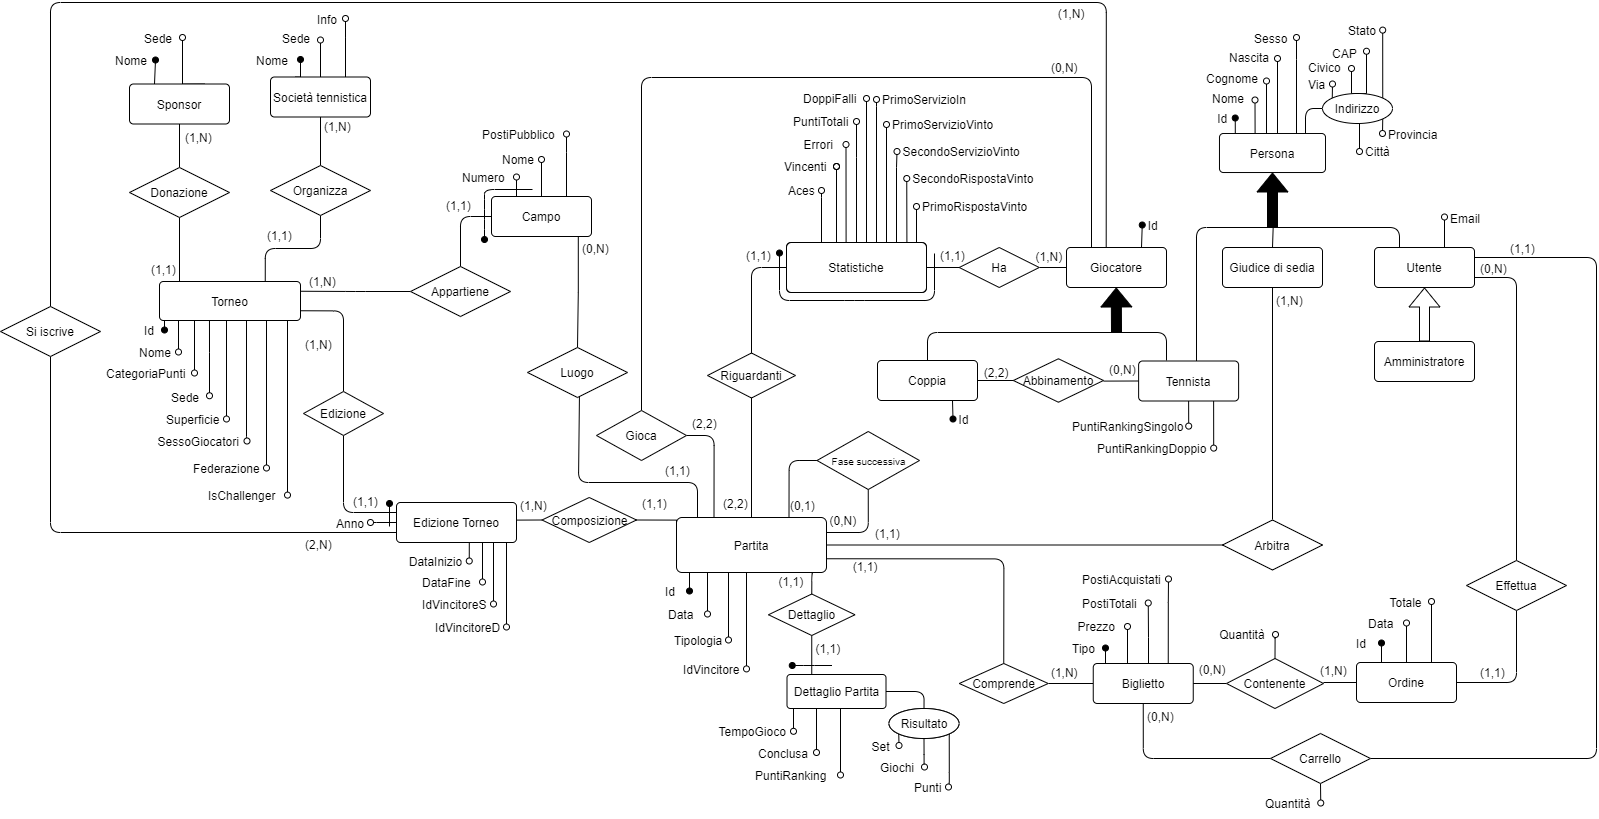
\includegraphics[width=1\textwidth]{images/BasiDati9.png}
}
\end{figure}

\section{Progettazione Logica}

\subsection{Ristrutturazione dello schema}

\subsubsection{Analisi delle ridondanze}

Una ridondanza è data dalla presenza dell'attributo \textit{tipologia} in partita, che può essere comunque ricavato dall'attributo con lo stesso nome presente in torneo: se il torneo è di quella tipologia, necessariamente lo saranno anche le partite presenti in esso.

Si sceglie di tenerli entrambi per avere l'informazione immediata già in partita.
\spazia

Un'altra ridondanza è nell'attributo \textit{totale} di ordine, che può essere ricavato sommando i vari attributi \textit{prezzo} di biglietto: si decide di mantenerlo, per non sovraccaricare il database, in quanto si stimano molte richieste giornaliere sulla tabella ordine.\spazia

La terza ridondanza è nella tabella campo: dato che si differenziano le entità torneo per genere maschile e femminile, si hanno delle ripetizioni di campi nel caso in cui per un torneo sia prevista anche la sua versione femminile nello stesso luogo. 

Tuttavia, questo non è sempre vero, in quanto sono 2 federazioni diverse ad occuparsi dell'organizzazione dei tornei e a volte capita di avere solo la versione maschile o femminile e non entrambe. La ridondanza, essendo parziale, deve quindi essere mantenuta. 

\subsubsection{Eliminazione delle generalizzazioni}
\begin{itemize}
    \item \underline{\textbf{Persona} $\longleftarrow$ Tennista, Giudice di sedia, Utente} \spazia
    Si risolve la generalizzazione totale creando tre tabelle: Tennista, Giudice di sedia, Utente, in quanto sono entità totalmente distinte, avendo funzionalità diverse.
    
    \item \underline{\textbf{Giocatore} $\longleftarrow$ Tennista, Coppia} \spazia
    Si risolve la generalizzazione totale creando due tabelle: Tennista e Coppia, in quanto sono entità che devono essere distinte e che hanno funzionalità diverse. Si aggiunge comunque un campo isCoppia in giocatore per identificare quando è una coppia.
    
    \item \underline{\textbf{Utente} $\Longleftarrow$ Amministratore} \spazia
    Si risolve la generalizzazione parziale semplicemente aggiungendo un campo bit \textit{isAdmin} a valore 1 quando l'utente è anche un amministratore del sito.
\end{itemize}

\subsubsection{Scelta degli identificatori primari}

Una scelta non banale è quella per l'identificatore primario di persona: in questo caso, si sarebbe potuto optare per 3 chiavi primarie: nome, cognome e data di nascita. Per riferirsi ad una qualsiasi persona, però sarebbe stato necessario utilizzare 3 chiavi esterne, che avrebbero portato ad un consumo eccessivo di memoria, rallentando il database. Si è scelto quindi di usare un identificativo univoco per ogni persona, riuscendo così a referenziarle più velocemente e facilmente.\spazia

Un'altra scelta simile è stata fatta per l'identificativo primario di partita: anche in questo caso, si sarebbe potuto scegliere di identificarla con gli id dei due giocatori che si scontrano e l'edizione del torneo in cui si svolge. Si è scelto comunque, come in precedenza, di usare un unico id per ogni partita, così da impedire l'uso eccessivo di memoria.\pagebreak

\subsubsection{Diagramma schema ristrutturato}
\begin{figure}[h]
\makebox[\textwidth][c]{
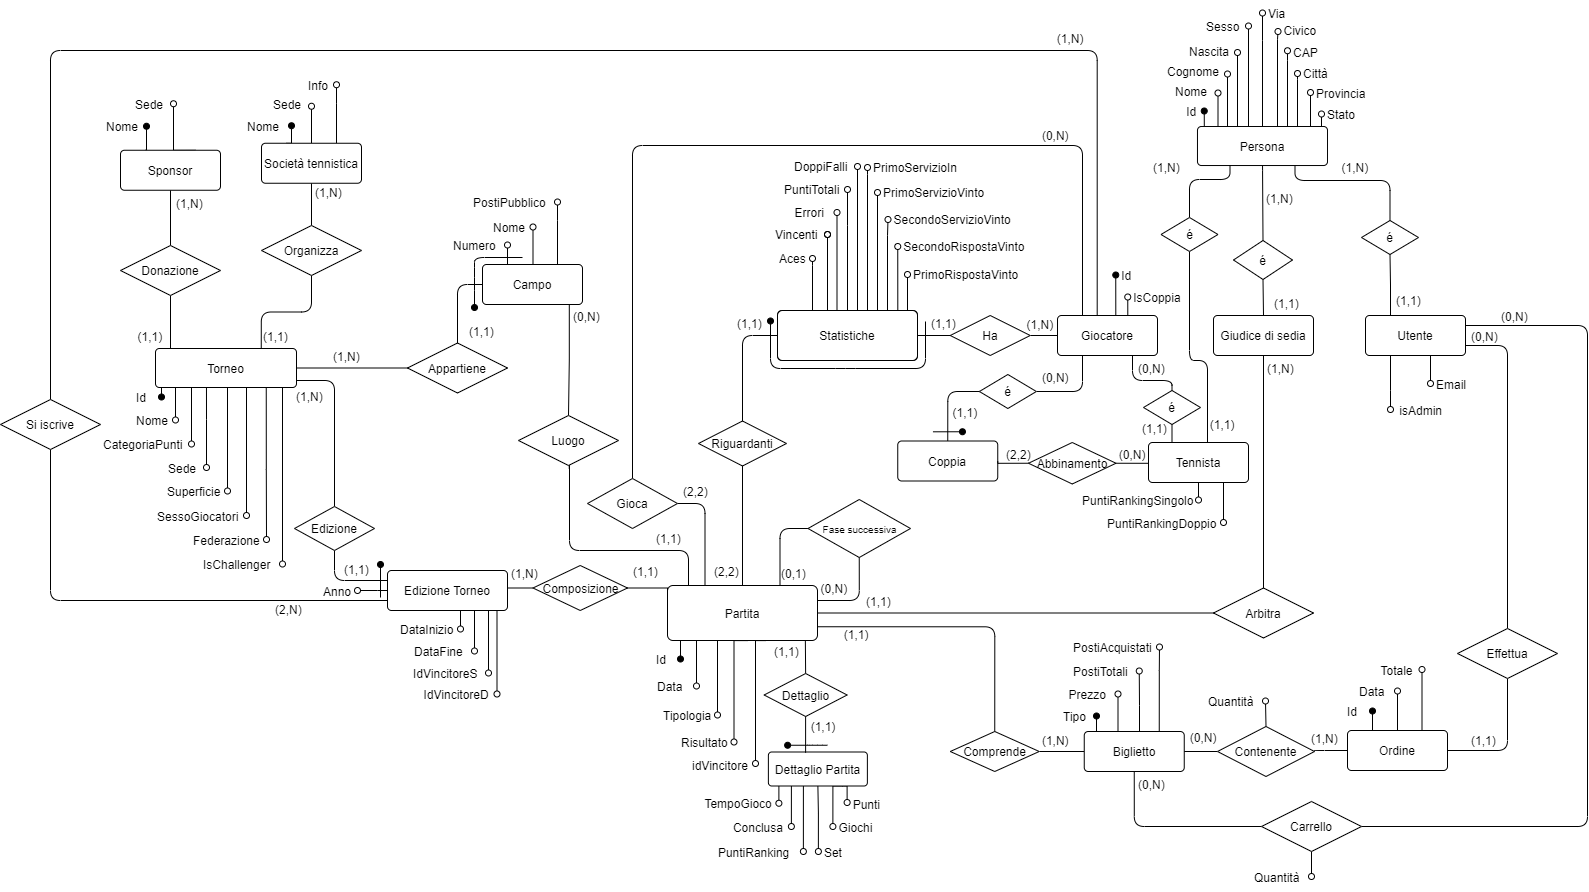
\includegraphics[width=1\textwidth]{images/BasiDatiRistrutturato4.png}
}
\end{figure}

\subsection{Schema relazionale}

\subsubsection{Descrizione Schema relazionale}
\begin{itemize}
    \item \textbf{Biglietto} (\underline{tipo}, prezzo, postiDisponibili, postiAcquistati)
    \item \textbf{Campo} (\underline{numero}, \underline{idTorneo}, nome, postiTifosi)
    \item \textbf{Giocatore} (\underline{id}, isCoppia)
    \item \textbf{Coppia} (\underline{idGiocatore}, tennista1, tennista2)
    \item \textbf{Ordine} (\underline{id}, data, totale)
    \item \textbf{Partita} (\underline{id}, data, tipologia, risultato, giocatore1, giocatore2, idPartitaFaseSucc, tipoBiglietto, idTorneo, annoTorneo, numeroCampo, idGiudiceDiSedia, idVincitore)
    \item \textbf{Dettaglio\_partita} (\underline{idPartita}, tempoGioco, conclusa, set, giochi, punti, puntiRanking)
    \item \textbf{Persona} (\underline{id}, nome, cognome, dataNascita, sesso, via, civico, CAP, stato, città, provincia)
    \item \textbf{Tennista} (\underline{idPersona}, idGiocatore, puntiRankingSingolo, puntiRankingDoppio)
    \item \textbf{Giudice\_di\_sedia} (\underline{id})
    \item \textbf{Utente} (\underline{id}, email, isAdmin)
    \item \textbf{Società\_tennistica} (\underline{nome}, sede, info)
    \item \textbf{Sponsor} (\underline{nome}, sede)
    \item \textbf{Statistiche} (\underline{idGiocatore}, \underline{idPartita}, aces, doppiFalli, puntiTot, errori, vincenti, primoServizioIn, primoServizioVinto, primoRispostaVinto, secondoServizioVinto, secondoRispostaVinto)
    \item \textbf{Torneo} (\underline{id}, nome, nomeSponsor, nomeSocieta, categoriaPunti, sede, superficie, sessoGiocatori, federazione, isChallenger)
    \item \textbf{Edizione\_torneo} (\underline{anno}, \underline{idTorneo}, dataInizio, dataFine, idVincitoreS, idVincitoreD)
    \item \textbf{Giocatore\_iscritto} (\underline{idGiocatore}, \underline{idTorneo}, \underline{annoTorneo})
    \item \textbf{Biglietti\_ordine} (\underline{tipoBiglietto}, \underline{idOrdine}, quantità)
    \item \textbf{Carrello} (\underline{tipoBiglietto}, \underline{idUtente}, quantità)
\end{itemize}

\subsubsection{Vincoli di integrità referenziale}
\begin{itemize}
    \item campo.idTorneo $\rightarrow$ torneo.id
    \item coppia.tennista1 $\rightarrow$ tennista.id
    \item coppia.tennista2 $\rightarrow$ tennista.id
    \item coppia.idGiocatore $\rightarrow$ giocatore.id
    \item partita.giocatore1 $\rightarrow$ giocatore.id
    \item partita.giocatore2 $\rightarrow$ giocatore.id
    \item partita.idPartitaFaseSuccessiva $\rightarrow$ partita.id
    \item partita.tipoBiglietto $\rightarrow$ biglietto.tipo
    \item partita.idTorneo $\rightarrow$ edizione\_torneo.idTorneo
    \item partita.annoTorneo $\rightarrow$ edizione\_torneo.anno
    \item partita.numeroCampo $\rightarrow$ campo.numero
    \item partita.idGiudiceDiSedia $\rightarrow$ giudice\_di\_sedia.id
    \item dettaglio\_partita.idPartita $\rightarrow$ partita.id
    \item tennista.idPersona $\rightarrow$ persona.id
    \item tennista.idGiocatore $\rightarrow$ giocatore.id
    \item giudice\_di\_sedia.id $\rightarrow$ persona.id
    \item utente.id $\rightarrow$ persona.id
    \item statistiche.idGiocatore $\rightarrow$ giocatore.id
    \item statistiche.idPartita $\rightarrow$ partita.id
    \item torneo.nomeSponsor $\rightarrow$ sponsor.nome
    \item torneo.nomeSocieta $\rightarrow$ societa\_tennistica.nome
    \item edizione\_torneo.idTorneo $\rightarrow$ torneo.id
    \item edizione\_torneo.idVincitoreS $\rightarrow$ giocatore\_iscritto.id
    \item edizione\_torneo.idvincitoreD $\rightarrow$ giocatore\_iscritto.id
    \item giocatore\_iscritto.idGiocatore $\rightarrow$ giocatore.id
    \item giocatore\_iscritto.idTorneo $\rightarrow$ edizione\_torneo.idTorneo
    \item giocatore\_iscritto.annoTorneo $\rightarrow$ edizione\_torneo.anno
    \item biglietti\_ordine.tipoBiglietto $\rightarrow$ biglietto.tipo
    \item biglietti\_ordine.idOrdine $\rightarrow$ ordine.id
    \item carrello.tipoBiglietto $\rightarrow$ biglietto.tipo
    \item carrello.idCarrello $\rightarrow$ carrello.idUtente
    \item ordine.idUtente $\rightarrow$ utente.id
\end{itemize}\spazia \spazia \spazia
\section{Query e Indici}
\spazia 
\subsection{Query}\spazia
1) Elencare i tornei disputati negli ultimi 12 mesi con relative informazioni quali la superficie la categoria di punti ranking a cui appartengono, la federazione, la sede e il vincitore.

\begin{figure}[h]
\makebox[\textwidth][c]{
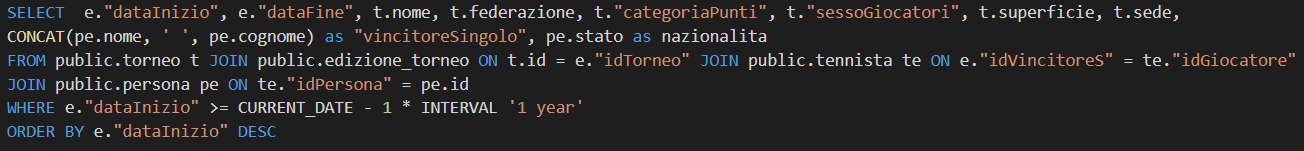
\includegraphics[width=1\textwidth]{images/QueryTornei.PNG}
}
\makebox[\textwidth][c]{
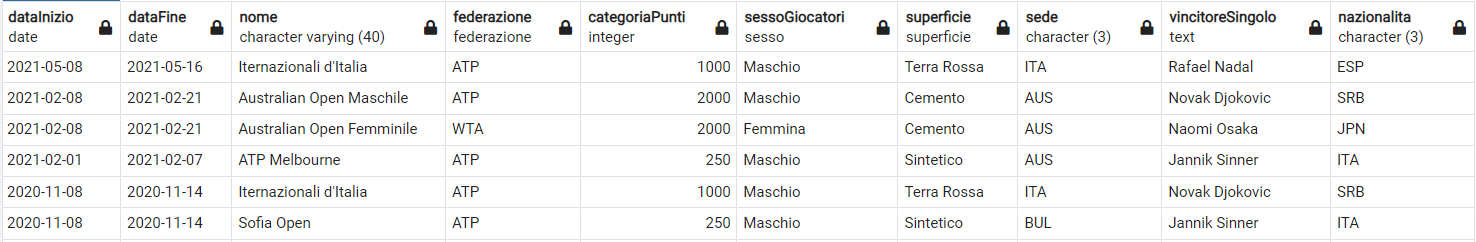
\includegraphics[width=1\textwidth]{images/QueryTorneiRisultati.PNG}
}
\end{figure}
\spazia

2) Elencare i 3 migliori giocatori per percentuale di punti vinti con un ace dall'inizio del 2020 in avanti.

\begin{figure}[h]
\makebox[\textwidth][c]{
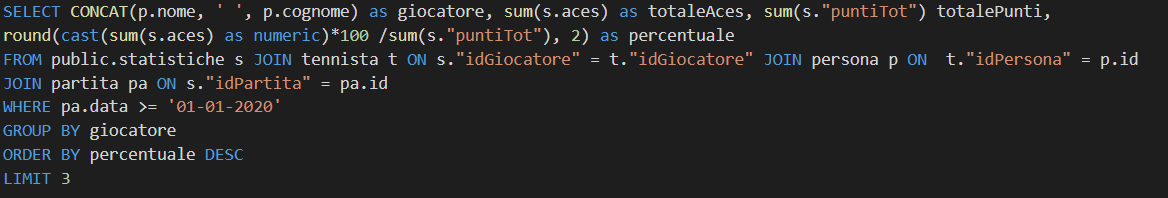
\includegraphics[width=1\textwidth]{images/QueryStatistiche.PNG}
}
\makebox[\textwidth][c]{
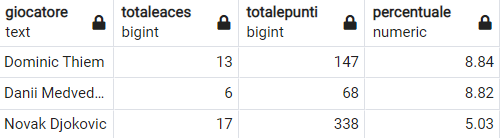
\includegraphics[width=0.5\textwidth]{images/QueryStatisticheRisultati.PNG}
}
\end{figure}
\spazia

3) Elencare i tennisti di una certa nazionalità (nell'esempio sono scelti i tennisti serbi) e le finali che hanno disputato in tornei ATP appartenenti al Tour principale, ovvero che hanno una categoria punti >=250.

\begin{figure}[h]
\makebox[\textwidth][c]{
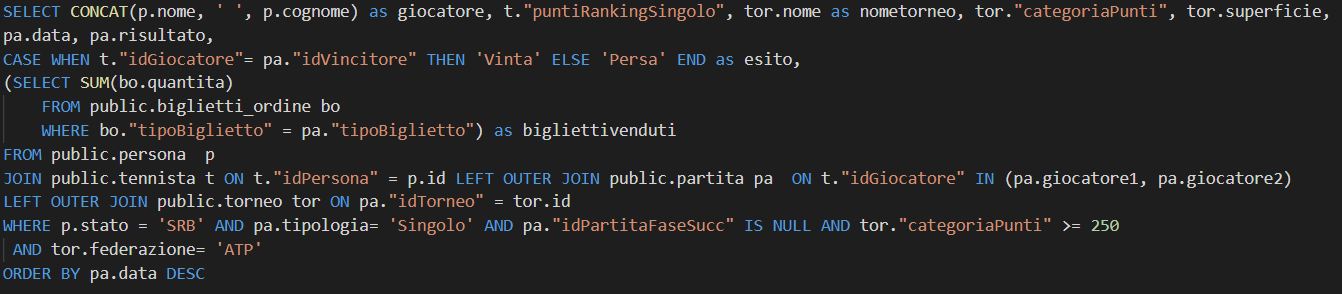
\includegraphics[width=1\textwidth]{images/QueryTennisti.PNG}
}
\makebox[\textwidth][c]{
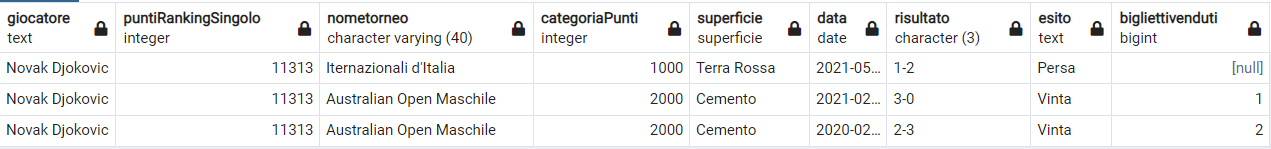
\includegraphics[width=1\textwidth]{images/QueryTennistiRisultati.PNG}
}
\end{figure}
\pagebreak

4) Elencare i tornei che hanno avuto più biglietti acquistati nel 2021 con il totale dei guadagni ottenuti da tali biglietti. \spazia \spazia 

\begin{figure}[h]
\makebox[\textwidth][c]{
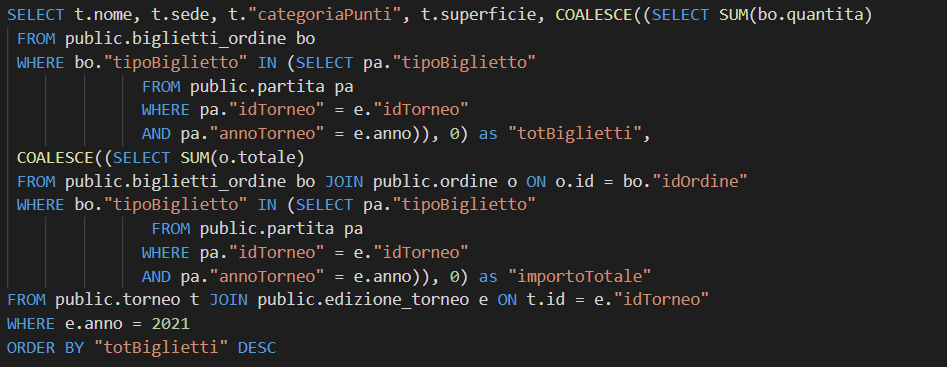
\includegraphics[width=1\textwidth]{images/QueryOrdini.PNG}
}
\makebox[\textwidth][c]{
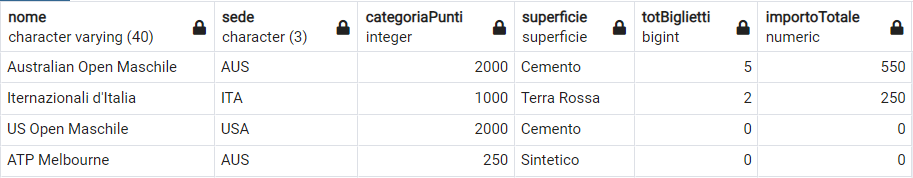
\includegraphics[width=1\textwidth]{images/QueryOrdiniRisultati.PNG}
}
\end{figure}
\spazia \spazia \spazia  \spazia 

5) Elencare tutti gli scontri avvenuti tra due tennisti a scelta con relativi dettagli delle partite \spazia \spazia 

\begin{figure}[h]
\makebox[\textwidth][c]{
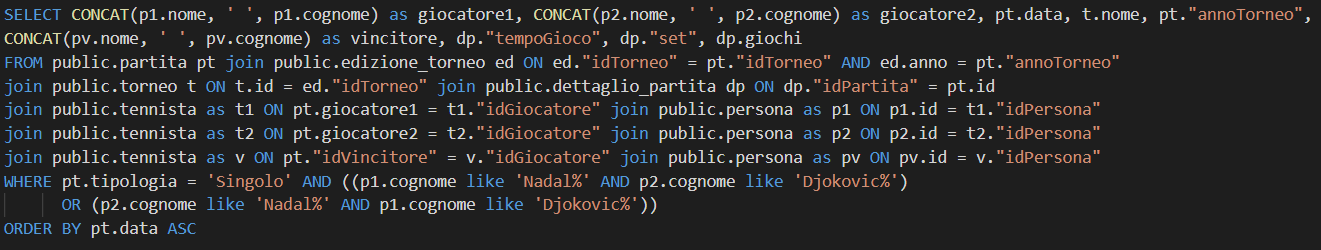
\includegraphics[width=1\textwidth]{images/QueryHeadToHead.PNG}
}
\makebox[\textwidth][c]{

\includegraphics[width=1\textwidth]{images/QueryHeadToHeadRisultati.PNG}
}
\end{figure}
\pagebreak
6) Elencare il tabellone delle fasi finali (dai quarti in poi) dell'edizione del 2020 dell'Australian Open Maschile con relativi giudici di sedia e campi in cui si sono disputate le partite.

\begin{figure}[h]
\makebox[\textwidth][c]{
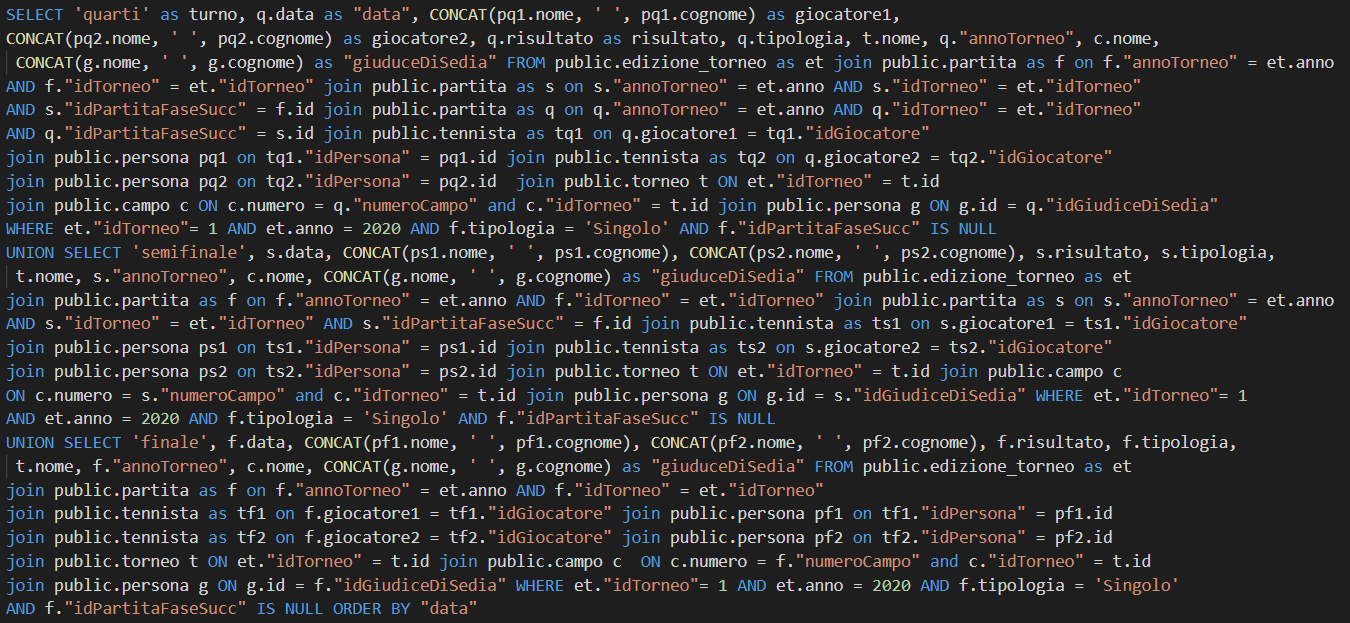
\includegraphics[width=1\textwidth]{images/QueryTabellone.PNG}
}
\makebox[\textwidth][c]{
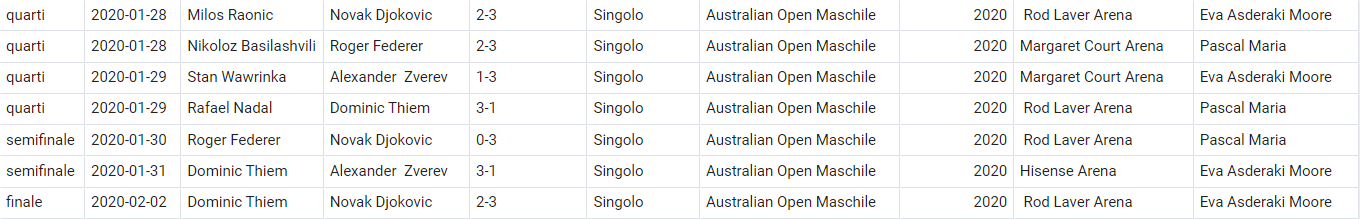
\includegraphics[width=1\textwidth]{images/QueryTabelloneRisultati.PNG}
}
\end{figure}

\subsection{Indici}
Nel corso del tempo, la tabella \textit{partita} aumenta di dimensioni, e contiene un numero sempre più elevato di tuple. Si ipotizza che la ricerca dei risultati finali sia un'operazione frequente, per cui si ritiene utile la definizione di un indice sul campo \textit{risultato}.
\begin{figure}[h]
\makebox[\textwidth][c]{

\includegraphics[width=0.7\textwidth]{images/Indice.PNG}
}
\end{figure}

\section{File in C++}

Si è scelto di usare due file \textit{.cpp}, uno per il main, dove vengono stampati i risultati e uno per le varie query, che vengono divise in funzioni diverse. Facendo così, si riutilizza la parte di codice che si occupa di stampare i risultati delle query e si dà una maggiore chiarezza separandole dal main.\spazia

Per produrre l'eseguibile è sufficiente compilare il file \textit{main.cpp}, ovviamente includendo la libreria \textit{libpq}.

L'eseguibile poi è stato strutturato in modo da guidare l'utente nell'operatività.

\section{Note}
Il database è stato popolato con un insieme di dati per la gran parte reali, minimale e tuttavia sufficiente a dimostrarne tutte le funzionalità.

\end{document}
